\documentclass[11pt]{article}
\usepackage{amssymb}
\usepackage{amsthm}
\usepackage{enumitem}
\usepackage{physics,amsmath}
\usepackage{bm}
\usepackage{adjustbox}
\usepackage{mathrsfs}
\usepackage{graphicx}
\usepackage{siunitx}
\usepackage[mathscr]{euscript}

\title{\textbf{Solved selected problems of Classical Mechanics - Gregory}}
\author{Franco Zacco}
\date{}

\addtolength{\topmargin}{-3cm}
\addtolength{\textheight}{3cm}

\newcommand{\hatr}{\bm{\hat{r}}}
\newcommand{\hatx}{\bm{\hat{x}}}
\newcommand{\haty}{\bm{\hat{y}}}
\newcommand{\hatz}{\bm{\hat{z}}}
\newcommand{\hatth}{\bm{\hat{\theta}}}
\newcommand{\hatphi}{\bm{\hat{\phi}}}
\newcommand{\hatrho}{\bm{\hat{\rho}}}
\theoremstyle{definition}
\newtheorem*{solution*}{Solution}
\renewcommand*{\proofname}{\bf{Solution}}

\begin{document}
\maketitle
\thispagestyle{empty}

\section*{Chapter 12 - Lagrange's equations and conservation principles}

\begin{proof}{\textbf{12.2}}
    The system described looks like the following
    \begin{center}
        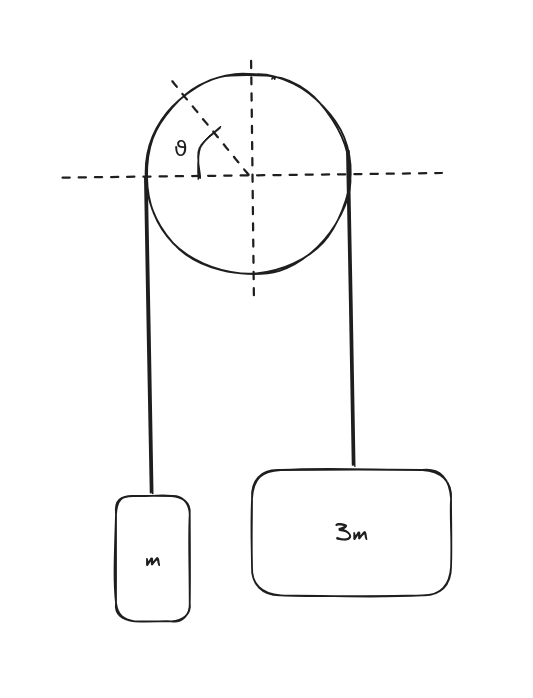
\includegraphics[scale=0.4]{ch12-2.png}
    \end{center}
    The system is a standard system and the forces are conservative so we can
    apply the Lagrange method for conservative systems where $\theta$ is our
    generalized coordinate.
    In this case, the kinetic energy is given by
    \begin{align*}
        T &= \frac{1}{2}(mr^2)\dot{\theta}^2 + \frac{1}{2}m(\dot\theta r)^2
        + \frac{1}{2}3m(\dot\theta r)^2\\
        T &= \frac{5}{2}mr^2\dot{\theta}^2
    \end{align*}
    Where the first term corresponds to the pulley and the last 2 to the
    masses hanging. Also, $r$ is the radius of the pulley.
    
    For the potential energy, we have that
    \begin{align*}
        V &= mg(\theta r) - 3mg(\theta r)\\
        V &= -2mg(\theta r)
    \end{align*}
    Now we compute the partial derivatives as follows
    \begin{align*}
        \frac{\partial T}{\partial \theta} = 0\quad\quad
        \frac{\partial T}{\partial \dot\theta} = 5mr^2\dot\theta\quad\quad
        \frac{\partial V}{\partial \theta} = -2mgr
    \end{align*}
    So the Lagrange equation is given by
    \begin{align*}
        \frac{d}{dt}(5mr^2\dot\theta) - 0 &= 2mgr\\
        r\ddot\theta &= \frac{2}{5}g
    \end{align*}
    Therefore the upward acceleration of the mass $m$ is $a = \frac{2}{5}g$
    since the mass is experiencing the same acceleration as the tangential
    acceleration of the pulley because of the no slipping restriction.
\end{proof}
\cleardoublepage
\begin{proof}{\textbf{12.3}}
    The system described looks like the following
    \begin{center}
        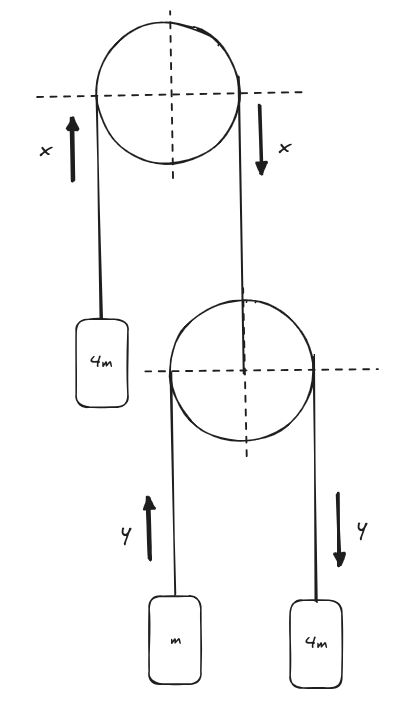
\includegraphics[scale=0.45]{ch12-3.png}
    \end{center}
    The system is a standard system and the forces are conservative so we can
    apply the Lagrange method for conservative systems where $x$ and
    $y$ (the displacements with respect to each pulley) are our generalized
    coordinates. In this case, the kinetic energy is given by
    \begin{align*}
        T &= \frac{1}{2}4m\dot{x}^2
        + \frac{1}{2}m(-\dot{x} + \dot{y})^2 + \frac{1}{2}4m(-\dot{x} - \dot{y})^2\\
        T &= \frac{1}{2}m(4\dot{x}^2 + \dot{x}^2 - 2\dot{x}\dot{y} + \dot{y}^2 
        + 4(\dot{x}^2 + 2\dot{x}\dot{y} + \dot{y}^2))\\
        T &= \frac{1}{2}m(9\dot{x}^2 + 6\dot{x}\dot{y} + 5 \dot{y}^2)
    \end{align*}
    For the potential energy, we have that
    \begin{align*}
        V &= 4mgx + mg(y-x) - 4mg(y+x)\\
        % V &= 4mgx + mgy - mgx - 4mgy - 4mgx
        V &= -mgx -3mgy
    \end{align*}
    Now we compute the partial derivatives as follows
    \begin{align*}
        \frac{\partial T}{\partial x} = 0\quad\quad
        \frac{\partial T}{\partial \dot x} = m(9\dot{x} + 3\dot{y})\quad\quad
        \frac{\partial V}{\partial x} = -mg\\\\
        \frac{\partial T}{\partial y} = 0\quad\quad
        \frac{\partial T}{\partial \dot y} = m(5\dot{y} + 3\dot{x})\quad\quad
        \frac{\partial V}{\partial y} = -3mg\\
    \end{align*}
    So the Lagrange equation for $q_1 = x$ is given by
    \begin{align*}
        \frac{d}{dt}(m(9\dot{x} + 3\dot{y})) - 0 &= mg\\
        9\ddot{x} + 3\ddot{y} &= g
    \end{align*}
    And for $q_2 = y$ we have that
    \begin{align*}
        \frac{d}{dt}(m(5\dot{y} + 3\dot{x})) - 0 &= 3mg\\
        5\ddot{y} + 3\ddot{x} &= 3g
    \end{align*}
    Therefore the generalized coordinates accelerations are
    \begin{align*}
        \ddot{y} = \frac{2}{3}g\quad\quad
        \ddot{x} = -\frac{g}{9}
    \end{align*}
    So the acceleration for the mass $4m$ of the upward pulley is
    $\ddot{x} = -g/9$, the acceleration for the mass $m$ of the downward pulley
    is $\ddot{y} - \ddot{x} = 7g/9$ and the acceleration for the mass $4m$
    of the downward pulley is $-\ddot{y} - \ddot{x} = -5g/9$.
\end{proof}
\cleardoublepage
\begin{proof}{\textbf{12.4}}
    The system described looks like the following
    \begin{center}
        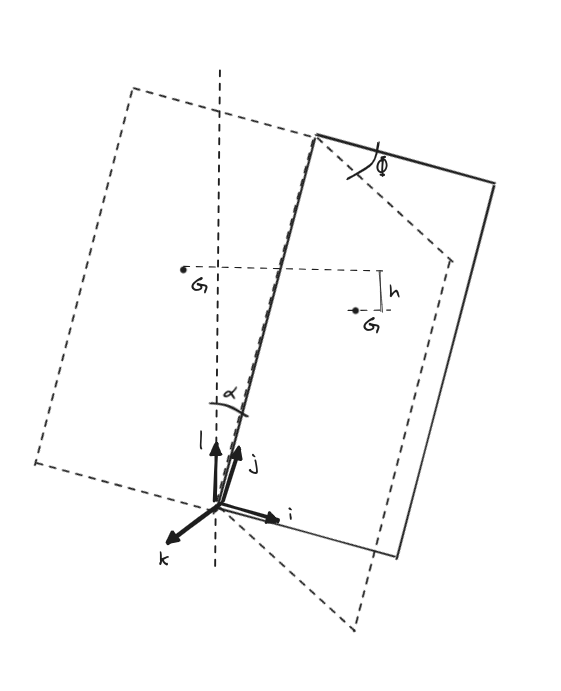
\includegraphics[scale=0.45]{ch12-4.png}
    \end{center}
    Where our generalized coordinate is $\phi$ the angle of rotation from the
    door equilibrium position.
    
    First, we need to compute the moment of inertia of
    the door with respect to the hinges, let $\rho = m/2a$  be
    the linear density of mass then a differential of mass is given by
    $dm = \rho dx$ hence 
    \begin{align*}
        I &= \int_0^{2a} \frac{mx^2}{2a} dx\\
        &= \frac{m}{2a} \bigg[\frac{x^3}{3}\bigg]_0^{2a}\\
        &= \frac{4}{3}ma^2
    \end{align*}
    So in this case, the kinetic energy is
    \begin{align*}
        T &= \frac{1}{2}\bigg(\frac{4}{3}ma^2\bigg) \dot\phi^2
        = \frac{2}{3}ma^2 \dot\phi^2 
    \end{align*}

    Now we have to compute the potential energy. Let us define a set of
    coordinates $\bm{i},\bm{j},\bm{k}$ where $\bm{i}$ and $\bm{j}$ are in the
    plane of the door equilibrium position and $\bm{k}$ is perpendicular to
    them. We need to determine first the height gain of the center of mass
    when the door is opened.
    Let the center of mass in the equilibrium position be
    $G = a \bm{i} + b\bm{j}$ then the center of mass will be at
    $G = a\cos\phi\bm{i} + b\bm{j} + a\sin\phi \bm{k}$ when
    the door is opened at an angle $\phi$ hence the center of mass of the door
    has displaced
    \begin{align*}
        \Delta G = a(\cos\phi - 1) \bm{i} + a\sin\phi \bm{k}
    \end{align*}
    But we are interested in the vertical component of this quantity  so we
    multiply this expression by $\bm{l}$ our vertical unit vector, so we get
    that
    \begin{align*}
        h = \Delta G\cdot\bm{l} &= a(\cos\phi - 1) \bm{i}\cdot \bm{l}
        + a\sin\phi \bm{k} \cdot \bm{l}\\
        &= a(\cos\phi - 1) \bm{i}\cdot \bm{l} + 0\\
        &= a(\cos\phi - 1) \cos(\alpha + \pi/2)\\
        &= -a(\cos\phi - 1) \sin(\alpha)
    \end{align*}
    Then the potential energy is given by:
    \begin{align*}
        V &= -mgh = mga(\cos\phi - 1) \sin(\alpha)
    \end{align*}
    Now we compute the partial derivatives as follows
    \begin{align*}
        \frac{\partial T}{\partial \phi} = 0\quad\quad
        \frac{\partial T}{\partial \dot \phi} = \frac{4}{3}ma^2 \dot\phi\quad\quad
        \frac{\partial V}{\partial \phi} = -mga\sin(\alpha)\sin\phi
    \end{align*}
    So the Lagrange equation for $q_1 = \phi$ is given by
    \begin{align*}
        \frac{d}{dt}(\frac{4}{3}ma^2 \dot\phi) - 0 &= mga\sin(\alpha)\sin\phi\\
        \frac{4}{3}a\ddot\phi &= g\sin(\alpha)\sin\phi\\
        \ddot\phi &= \frac{3}{4}\frac{g\sin(\alpha)}{a}\sin\phi\\
        \ddot\phi - \frac{3}{4}\frac{g\sin(\alpha)}{a}\sin\phi &= 0
    \end{align*}
    But when $\phi$ is small we can assume $\sin\phi \approx \phi$ so we get
    \begin{align*}
        \ddot\phi - \frac{3}{4}\frac{g\sin(\alpha)}{a}\phi &= 0
    \end{align*}
    Which is the equation for a simple harmonic motion of the form
    $\ddot{x} + \Omega^2 x =0$ where we know the period
    is given by $\tau = 2\pi / \Omega$ therefore
    the period of small oscillations is
    \begin{align*}
        \tau = \frac{2\pi}{\sqrt{\frac{3}{4}\frac{g\sin(\alpha)}{a}}} 
        = 2\pi \sqrt{\frac{4a}{3g \sin \alpha}}
    \end{align*}
\end{proof}
\cleardoublepage
\begin{proof}{\textbf{12.6}}
    The system described looks like the following
    \begin{center}
        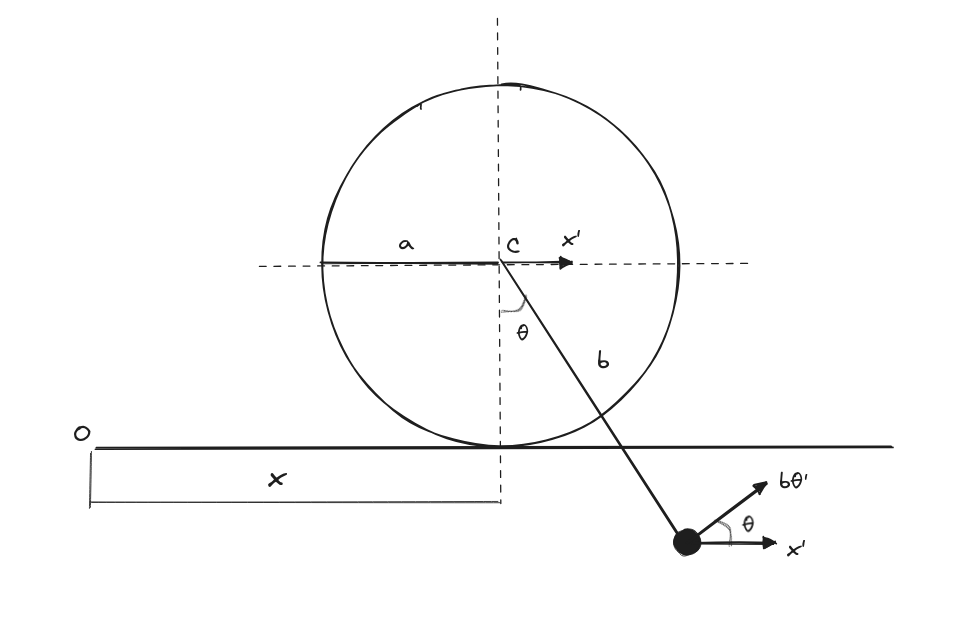
\includegraphics[scale=0.45]{ch12-6.png}
    \end{center}
    Where our generalized coordinates are $x$ and $\theta$.
    The kinetic energy in this case is given by
    \begin{align*}
        T &= \frac{1}{2}M \dot x^2
        + \frac{1}{2}\bigg(\frac{1}{2}Ma^2\bigg) \bigg(\frac{\dot{x}}{a}\bigg)^2
        + \frac{1}{2}m\bigg(b\dot\theta + \dot x\bigg)^2\\
        T &= \frac{3}{4}M\dot{x}^2 + \frac{1}{2}m\bigg(b^2\dot{\theta}^2
        + 2b\dot\theta\dot x\cos\theta
        + \dot x^2\bigg) 
    \end{align*}
    Where we used that the angular velocity of the disk is $\dot{x}/a$ because
    of the rolling condition. 
    Now we determine the potential energy, there is no change in the height
    for the center of mass of the disk but there is for the hanging mass hence
    \begin{align*}
        V &= - mgb\cos\theta
    \end{align*}
    Then the Lagrangian is
    \begin{align*}
        L = T - V &= \frac{3}{4}M\dot{x}^2 + \frac{1}{2}m\bigg(b^2\dot{\theta}^2
        + 2b\dot\theta\dot x\cos\theta
        + \dot x^2\bigg) + mgb\cos\theta
    \end{align*}
    We see that $L$ is not a function of $x$ hence $x$ is a cyclic coordinate.
    The generalized momentum $p_x$ is given by
    \begin{align*}
        p_x = \frac{\partial L}{\partial \dot{x}} = 
        \frac{3}{2}M\dot{x} + m\bigg(b\dot\theta\cos\theta + \dot x\bigg)
    \end{align*}
    And it's not the horizontal linear momentum which is given by
    \begin{align*}
        M\dot{x} + m\bigg(b\dot\theta\cos\theta + \dot x\bigg)
    \end{align*}

    Finally, we compute the Lagrangian partial derivatives left
    \begin{align*}
        \frac{\partial L}{\partial \dot\theta} &= mb(b\dot{\theta}
        + \dot x\cos\theta)\\
        \frac{\partial L}{\partial \theta} &= -mb\dot\theta\dot x\sin\theta 
        -mbg\sin\theta 
    \end{align*}
    So now we compute the Lagrangian form for the two generalized coordinates
    as follows
    \begin{align*}
        \frac{d}{dt}\bigg(\frac{\partial L}{\partial \dot\theta}\bigg)
        - \frac{\partial L}{\partial \theta} &= 0\\
        mb(b\ddot{\theta} + \ddot x\cos\theta - \dot x\dot\theta\sin\theta)
        + mb\dot\theta\dot x\sin\theta  + mbg\sin\theta &= 0\\
        b\ddot{\theta} + \ddot x\cos\theta 
        + g\sin\theta &= 0\\
    \end{align*}
    and 
    \begin{align*}
        \frac{d}{dt}\bigg(\frac{\partial L}{\partial \dot x}\bigg) - 0 &= 0\\
        \frac{3}{2}M\ddot{x}
        + m\bigg(b(\ddot\theta\cos\theta
        - \dot\theta^2\sin\theta) + \ddot x\bigg) &= 0\\
        \ddot{x}\bigg(\frac{3}{2}M + m\bigg)
        + mb(\ddot\theta\cos\theta
        - \dot\theta^2\sin\theta) &= 0\\
        -\frac{mb}{\frac{3}{2}M + m}(\ddot\theta\cos\theta
        - \dot\theta^2\sin\theta) &= \ddot x
    \end{align*}
    By replacing $\ddot x$ we get that
    \begin{align*}
        b\ddot{\theta}
        - \frac{mb\cos\theta}{\frac{3}{2}M + m}(\ddot\theta\cos\theta
        - \dot\theta^2\sin\theta)
        + g\sin\theta &= 0\\
        \ddot{\theta}
        - \frac{2m\cos\theta}{(3M + 2m)}(\ddot\theta\cos\theta
        - \dot\theta^2\sin\theta)
        + \frac{g}{b}\sin\theta &= 0\\
        \ddot{\theta}\bigg( 
        1 - \frac{2m\cos^2\theta}{(3M + 2m)}\bigg)
        + \frac{2m\cos\theta\sin\theta}{(3M + 2m)}\dot\theta^2
        + \frac{g}{b}\sin\theta &= 0\\
        \ddot{\theta}(3M + 2m\sin^2\theta)
        + 2m\cos\theta\sin\theta\dot\theta^2
        + \frac{g(3M + 2m)}{b}\sin\theta &= 0
    \end{align*}
    Now we approximate this equation to a linear equation by neglecting
    quadratic terms (i.e. $\theta^2$ and $\dot\theta^2$) and assuming
    $\cos\theta \approx 1$ and $\sin\theta \approx \theta$ hence the
    linearized equation is
    \begin{align*}
        \ddot{\theta} + \frac{g(3M + 2m)}{3Mb} \theta &= 0
    \end{align*}
    Therefore the period of small oscillations is given by
    \begin{align*}
        \tau &= 2\pi\sqrt{\frac{3Mb}{g(3M + 2m)}}
    \end{align*}
\end{proof}
\begin{proof}{\textbf{12.7}}
    The system described looks like the following
    \begin{center}
        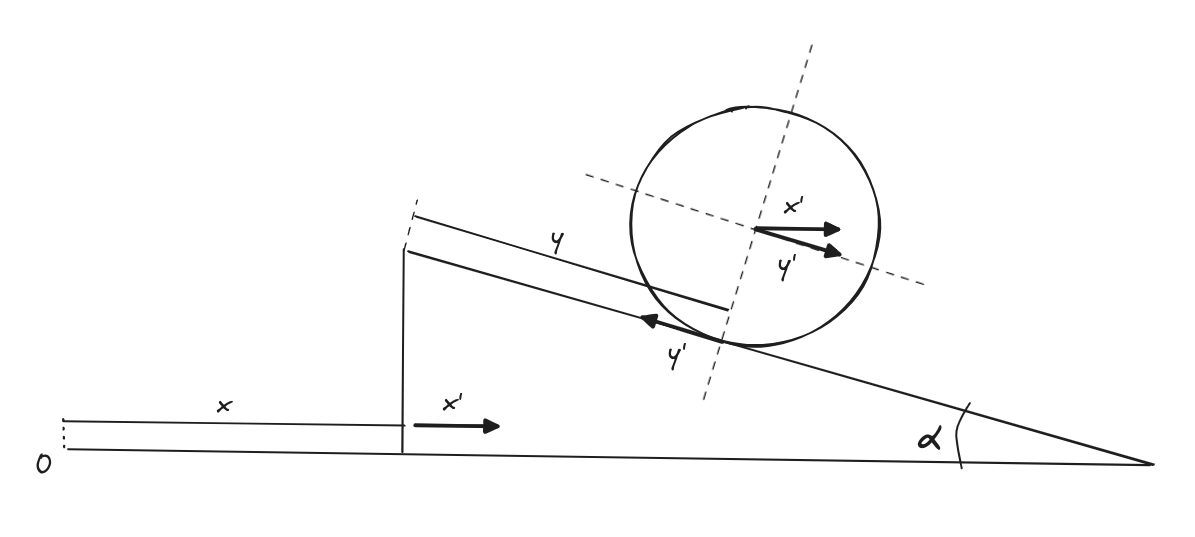
\includegraphics[scale=0.4]{ch12-7.png}
    \end{center}
    Where our generalized coordinates are $x$ and $y$ hence we have 2 degrees
    of freedom. The kinetic energy in this case is given by
    \begin{align*}
        T &= \frac{1}{2}M \dot x^2
        + \frac{1}{2}\bigg(\frac{2}{5}ma^2\bigg) \bigg(\frac{\dot{y}}{a}\bigg)^2
        + \frac{1}{2}m\bigg(\dot y + \dot x\bigg)^2\\
        T &= \frac{1}{2}M\dot{x}^2 + \frac{1}{5}m\dot y^2
        + \frac{1}{2}m(\dot x^2 + 2\dot x\dot y\cos\alpha + \dot y^2)
        % T &= \frac{1}{2}M\dot{x}^2 + \frac{1}{5}m\dot y^2
        % + \frac{1}{2}m(\dot x^2 + 2\dot x\dot y\cos\theta + \dot y^2)
    \end{align*}
    Where we used that the angular velocity of the ball is $\dot{y}/a$ because
    of the rolling condition. Then the potential energy is
    \begin{align*}
        V &= - mgy\sin\alpha
    \end{align*}
    Now we compute the partial derivatives of $T$ and $V$ as follows
    \begin{align*}
        \frac{\partial T}{\partial x} = 0 \quad\quad&
        \frac{\partial T}{\partial \dot x} = \dot x (M + m) + m\dot y\cos\alpha\\
        \frac{\partial T}{\partial y} = 0 \quad\quad&
        \frac{\partial T}{\partial \dot y} =
        \frac{7}{5}m\dot{y} + m\dot x\cos\alpha\\
        \frac{\partial V}{\partial x} = 0 \quad\quad&
        \frac{\partial V}{\partial y} = -mg\sin\alpha
    \end{align*}
    So the Lagrange equation for $x$ gives us
    \begin{align*}
        \ddot x (M + m) + m\ddot y\cos\alpha &= 0
    \end{align*}
    And for $y$
    \begin{align*}
        \frac{7}{5}m\ddot{y} + m\ddot x\cos\alpha &= mg\sin\alpha\\
        \frac{7}{5}\ddot{y} + \ddot x\cos\alpha &= g\sin\alpha
    \end{align*}
    If we assume now $M = 3m/2$ we get from the $x$-Lagrange equation that
    \begin{align*}
        \frac{5}{2}\ddot x + \ddot y\cos\alpha &= 0
    \end{align*}
    the second Lagrange equation does not depend on $M$ so it's left untouched. 
    Then by replacing the values, we get that the acceleration of the wedge is
    \begin{align*}
        -\frac{7}{2}\frac{\ddot x}{\cos\alpha} + \ddot x\cos\alpha &= g\sin\alpha\\
        -\frac{7}{2}\ddot x + \ddot x\cos^2\alpha &= g\sin\alpha\cos\alpha\\
        \ddot x &= \frac{2g\sin\alpha\cos\alpha}{2\cos^2\alpha - 7}
    \end{align*}
    In the same way, the acceleration of the ball with respect to the wedge is
    \begin{align*}
        \ddot y &=
        -\frac{5}{2\cos\alpha}\frac{2g\sin\alpha\cos\alpha}{2\cos^2\alpha - 7}\\
        \ddot y &= \frac{5g\sin\alpha}{7-2\cos^2\alpha}
    \end{align*}
\end{proof} 
\cleardoublepage
\begin{proof}{\textbf{12.9}}
    The system described looks like the following
    \begin{center}
        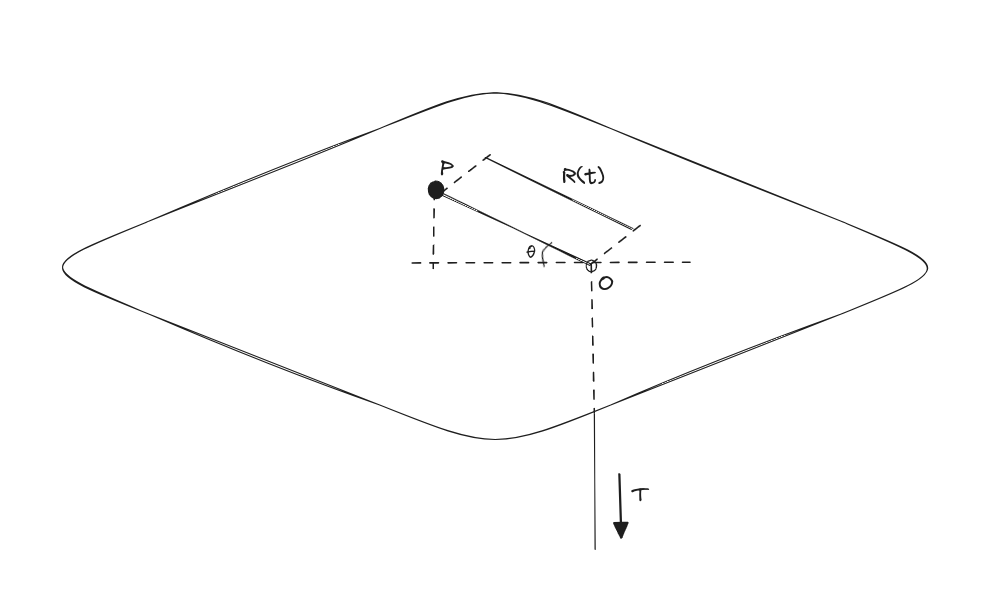
\includegraphics[scale=0.4]{ch12-9.png}
    \end{center}
    Where our generalized coordinate is $\theta$. We know that the velocity in
    polar coordinates is given by
    \begin{align*}
        v = \dot{R(t)} \hat{r} + R(t) \dot\theta \hat{\theta}
    \end{align*}
    hence the kinetic energy in this case is
    \begin{align*}
        T &= \frac{1}{2}m (\dot{R(t)} \hat{r} + R(t) \dot\theta \hat{\theta})^2\\
        T &= \frac{1}{2}m [\dot{R(t)}^2 + R(t)^2 \dot\theta^2]
    \end{align*}
    The kinetic energy is not conserved since the tension force is doing work
    on the particle.
    There is no change in the height of $P$ therefore the potential energy is
    $V = 0$. Then the Lagrangian is
    \begin{align*}
        L = T - V = \frac{1}{2}m [\dot{R(t)}^2 + R(t)^2 \dot\theta^2]
    \end{align*}
    We see that $L$ is not a function of $\theta$ hence $\theta$ is a cyclic
    coordinate. The generalized momentum $p_\theta$ is given by
    \begin{align*}
        p_\theta = \frac{\partial L}{\partial \dot\theta} 
        = m R(t)^2 \dot\theta
    \end{align*}
    From Newton's equations, we know that $F = ma$ where $F$ is the tension 
    in the string so if we write the acceleration in polar coordinates
    and we replace $\dot\theta = L/R(t)^2$ (since $mL = mR(t)^2\dot\theta$)
    we have that
    \begin{align*}
        F &= m[(\ddot{R} - R\dot{\theta}^2)\hat{r}
        + (R\ddot\theta + 2\dot{R}\dot\theta)\hat{\theta}]\\
        F &= m\bigg[\bigg(\ddot{R}
        - R\bigg(\frac{L^2}{R^4}\bigg)\bigg)\hat{r}
        + \bigg(-R\frac{2\dot{RL}}{R^3} + 2\dot{R}\frac{L}{R^2}\bigg)
        \hat{\theta}\bigg]\\
        F &= m\bigg(\ddot{R} 
        - \bigg(\frac{L^2}{R^3}\bigg)\bigg)\hat{r}
    \end{align*}

\end{proof}
\cleardoublepage
\begin{proof}{\textbf{12.10}}
    The system described looks like the following
    \begin{center}
        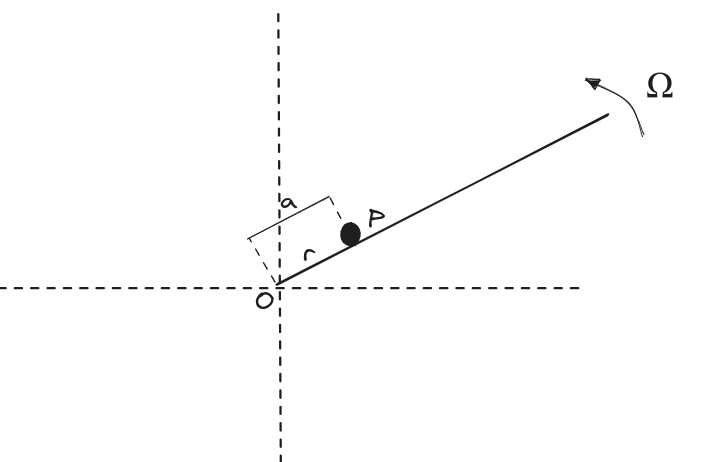
\includegraphics[scale=0.4]{ch12-10.png}
    \end{center}
    Where our generalized coordinate is $r$. The kinetic energy in this case is
    \begin{align*}
        T &= \frac{1}{2}m \dot{r}^2 + \frac{1}{2}m (\Omega r)^2
    \end{align*}
    Since gravity is not present then the potential energy for $P$ is $0$ hence
    the lagrangian is equal to $T$ i.e.
    \begin{align*}
        L &= \frac{1}{2}m (\dot{r}^2 + \Omega^2 r^2)
    \end{align*}
    Then the Lagrange equation is given by
    \begin{align*}
        \frac{d}{dt}\bigg(\frac{\partial L}{\partial \dot{r}}\bigg) - \frac{\partial L}{\partial r} &= 0\\
        \frac{d}{dt}\bigg(m\dot{r}\bigg) - m\Omega^2 r &= 0\\
        \ddot{r} - \Omega^2 r &= 0
    \end{align*}
    The solution for this differential equation and its derivative are
    \begin{align*}
        r &= A e^{\Omega t} + B e^{-\Omega t}\\
        \dot{r} &= A\Omega e^{\Omega t} - B\Omega e^{-\Omega t}
    \end{align*}
    we know from the initial conditions that $r = a$ and $\dot{r} = 0$ when
    $t = 0$ hence
    \begin{align*}
        a &= A + B\\
        0 &= A - B
    \end{align*}
    This implies that $B = A = a/2$ therefore the position of the particle at
    time $t$ is 
    \begin{align*}
        r &= \frac{a}{2}\bigg(e^{\Omega t} + e^{-\Omega t}\bigg)
        = a\cosh(\Omega t)
    \end{align*}
    Finally, the $h$ function is given by
    \begin{align*}
        h &= \frac{\partial L}{\partial \dot{r}} \dot{r} - L\\
        h &= m\dot{r}^2 - \frac{1}{2}m (\dot{r}^2 + \Omega^2 r^2)\\
        h &= \frac{1}{2}m (\dot{r}^2 - \Omega^2 r^2)
    \end{align*}
    If we replace $r$ and $\dot{r}$ we have that
    \begin{align*}
        h &= \frac{1}{2}m ((\Omega a\sinh(\Omega t))^2 - \Omega^2 (a\cosh(\Omega t))^2)\\
        h &= \frac{1}{2}m\Omega^2a^2(\sinh^2(\Omega t) -\cosh^2(\Omega t))\\
        h &= -\frac{1}{2}m\Omega^2a^2
    \end{align*}
    We see that $-\frac{1}{2}m\Omega^2a^2$ is a constant.
    Therefore the energy function is conserved.
\end{proof}
\cleardoublepage
\begin{proof}{\textbf{12.11}}
    The system described looks like the following
    \begin{center}
        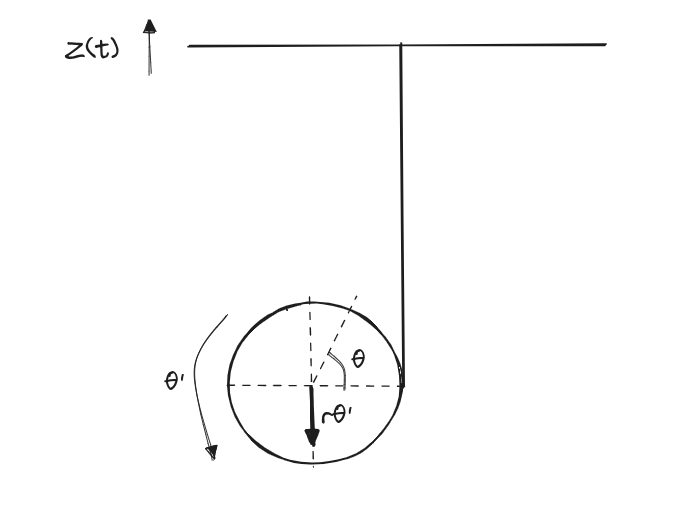
\includegraphics[scale=0.45]{ch12-11.png}
    \end{center}
    Where our generalized coordinate is $\theta$.
    Using the rolling condition of the yo-yo the kinetic energy in this case is
    \begin{align*}
        T &= \frac{1}{2}m(\bm{\bm{\dot{Z}} - r \dot{\theta}})^2
        + \frac{1}{2}\bigg(\frac{1}{2}mr^2\bigg)\bm{\dot{\theta}}^2\\
        T &= \frac{1}{2}m(\dot{Z}^2 - 2r\dot{\theta}\dot{Z} + (r \dot{\theta})^2)
        + \frac{1}{4}m(r\dot{\theta})^2\\
        T &= \frac{1}{2}m(\dot{Z}^2 - 2r\dot{\theta}\dot{Z})
        + \frac{3}{4}m(r\dot{\theta})^2
    \end{align*}
    The potential energy in this case is
    \begin{align*}
        V &= mg(Z - r\theta)
    \end{align*}
    Then the Lagrange equation is given by
    \begin{align*}
        \frac{d}{dt}\bigg[\frac{\partial T}{\partial \dot{\theta}}\bigg] - 
        \frac{\partial T}{\partial \theta}
        &= -\frac{\partial V}{\partial \theta}\\
        \frac{d}{dt}\bigg[
            -mr\dot{Z} + \frac{3}{2}mr^{2}\dot{\theta}
        \bigg] - 0 &= mgr\\
        -\ddot{Z} + \frac{3}{2}r\ddot{\theta} &= g
    \end{align*}
    So the acceleration of the yo-yo is
    \begin{align*}
        r\ddot{\theta} &= \frac{2}{3}(\ddot{Z} + g)
    \end{align*}
    The acceleration that the support must have so the center of the
    yo-yo can remain at rest can be determined by derivating the velocity of
    the yo-yo where $v = \dot{Z} - r \dot{\theta}$ i.e. 
    \begin{align*}
        a &= \ddot{Z} - r\ddot{\theta}\\
        &= \ddot{Z} - \frac{2}{3}(\ddot{Z} + g)\\
        &= \frac{\ddot{Z} - 2g}{3}
    \end{align*}
    This implies that the support must have an acceleration of $\ddot{Z} = 2g$
    so that the center of the yo-yo can remain at rest.
    
    If the whole system starts from rest then by integrating the yo-yo
    acceleration twice we get that
    \begin{align*}
        r\dot\theta = \frac{2}{3}(\dot{Z} + gt) + C_1
        \quad\quad\quad
        r\theta = \frac{2}{3}\bigg(Z + \frac{1}{2}gt^2\bigg) + C_2
    \end{align*}
    and since $\theta = \dot\theta = Z = \dot{Z} = 0$ when $t=0$ we see that
    $C_1 = C_2 = 0$ hence
    \begin{align*}
        r\dot\theta = \frac{2}{3}(\dot{Z} + gt)
        \quad\quad\quad
        r\theta = \frac{2}{3}\bigg(Z + \frac{1}{2}gt^2\bigg)
    \end{align*}
    Now if we replace these values in $T$ and $V$ we get that $E = T + V$ for
    some time $t$ is given by
    \begin{align*}
        E &= \frac{1}{2}m(\dot{Z}^2 - 2r\dot{\theta}\dot{Z})
        + \frac{3}{4}m(r\dot{\theta})^2 + mg(Z - r\theta)\\
        E &= \frac{1}{2}m(\dot{Z}^2 - \frac{4}{3}(\dot{Z} + gt)\dot{Z})
        + \frac{3}{4}m(\frac{2}{3}(\dot{Z} + gt))^2
        + mg\bigg(Z - \frac{2}{3}\bigg(Z + \frac{1}{2}gt^2\bigg)\bigg)\\
        E &= \frac{1}{2}m(-\frac{1}{3}\dot{Z}^2 - \frac{4}{3}gt\dot{Z})
        + \frac{1}{3}m(\dot{Z}^2 + 2\dot{Z}gt + (gt)^2)
        + mg\bigg(\frac{1}{3}Z - \frac{1}{3}gt^2\bigg)\\
        E &= m\bigg[-\frac{1}{6}\dot{Z}^2 - \frac{2}{3}gt\dot{Z}
        + \frac{1}{3}\dot{Z}^2 + \frac{2}{3}\dot{Z}gt + \frac{1}{3}(gt)^2
        + \frac{1}{3}gZ - \frac{1}{3}g^2t^2\bigg]\\
        E &= m\bigg[\frac{1}{6}\dot{Z}^2
        + \frac{1}{3}gZ\bigg] = m \bigg[\frac{\dot{Z}^2 + 2gZ}{6}\bigg]
    \end{align*}




\end{proof}

\end{document}






















